\chapter{Metodología de trabajo multidisciplinar}
\label{ch:metodologia}

Este capítulo describe la metodología de trabajo que se ha seguido para llevar a cabo el proyecto. Detalla las tareas y actividades que se planean realizar, así como el conjunto de herramientas de trabajo que se han visto con mayor utilidad para lograr un flujo de trabajo más productivo.\\

Como se mencionó anteriormente, mi tarea consistirá no solo en el desarrollo de una plataforma web, sino también la gestión del equipo, a modo de \textit{project manager}. Como tal, nos encontramos ante la situación de organizar a un equipo de personas que mayormente no son del mismo grado, por lo que pueden no estar acostumbrados o ser conocedores de las mismas herramientas que utlizamos habitualmente.\\

En el presente capítulo se tratará de buscar aquellas herramientas que sean sencillas y tengan una curva de aprendizaje baja. El motivo es múltiple, ya que se han de encontrar recursos aptos para todos, que no los abrumen o les frustren, para que así los utilicen y beneficie al proyecto en si.

\section{Líneas de trabajo}
En el nacimiento de este equipo, se planteó que debemos funcionar de forma similar a una Startup \cite{startup}. Siguiendo esa lógica, trabajamos sobre una idea innovadora para resolver un problema complejo, empleando la tecnología para llegar a cumplir el objetivo.\\

Sobre el concepto de SmartU, nacen una serie de \textbf{líneas de trabajo} que son importantes para lograr un producto completo y útil para su público objetivo, por ello es necesario que se trabaje en ellas de forma correcta.

\begin{description}
    \item[Software] La línea de trabajo donde crear aplicaciones web y móviles que el público objetivo usará con el fin de facilitar la tarea de la creación de proyectos multidisciplinares.
    \item[Marketing] Esta línea de trabajo concentra sus esfuerzos en la búsqueda de formas de promoción adecuadas al público y que garanticen que SmartU llegue al máximo número de personas posibles. Destacamos por ejemplo el uso de las redes institucionales ya existentes para dar difusión, así como la creación de redes sociales propias de la plataforma como forma de acercamiento a los demás.
    \item[Diseño gráfico] La identidad visual es el reto al que se enfrenta esta línea de trabajo. Se ha de encontrar un estilo y diseño diferenciador que además sea agradable al usuario, y que de alguna forma represente los conceptos sobre los que trabajamos, como por ejemplo el concepto principal de ciudades inteligentes.
    \item[Plan de empresa] El plan de empresa tiene como objetivo encontrar una estrategia de negocio que sirva para que esta \textit{startup} sea viable en el futuro.
\end{description}

\section{El equipo}
El equipo de trabajo se ha compuesto de diferentes \textbf{profesores y estudiantes} de diversas disciplinas de la universidad. Podemos ver su nombre y ocupación en la \textbf{tabla \ref{miembrossmartu}}. Todos han aportado conocimientos de su campo al proyecto para intentar lograr los mejores resultados, recibiendo opiniones y puntos de vista muy diferentes que ayudan y complementan.

\begin{table}
    \begin{center}
        \begin{tabular}{|p{4.5cm}|p{6.5cm}|}
            \hline
                \rowcolor{Gray}\multicolumn{1}{|c|}{\textbf{Integrante}}
                & \multicolumn{1}{|c|}{\textbf{Ocupación}} \\
            \hline
                Juan Árbol Gutiérrez & Estudiante de CC.EE. y Empresariales \\
            \hline
                Irene Castillo Pardo & Estudiante de Comunicación y Audiovisuales \\
            \hline
                Emilio Chica Jiménez & Estudiante de Ingeniería Informática \\
            \hline
                Victoria Guerra Molina & Estudiante de Comunicación y Audiovisuales \\
            \hline
                Juan José Jiménez García & Estudiante de Ingeniería Informática \\
            \hline
                Javier Labrat Rodríguez & Estudiante de Ingeniería Informática \\
            \hline
                Germán Zayas Cabrera & Estudiante de Bellas Artes \\
            \hline
                Miguel Gea Megías & Profesor de Ingeniería Informática \\
            \hline
                Guillermo Maraver Tarifa & Profesor de CC.EE. y Empresariales \\
            \hline
                Alejandro Grindlay Moreno & Profesor de Ingeniería Civil \\
            \hline
        \end{tabular}
        \caption{Integrantes del proyecto multidisciplinar SmartU}
        \label{miembrossmartu}
    \end{center}
\end{table}

\subsection{Obligaciones del equipo}
A cada uno de los miembros del equipo se le asigna un rol o tarea. Es importante que cada uno se dedique a algo relacionado con sus conocimientos, de esta manera se esperaba conseguir mejores resultados, al \textbf{delegar en la persona adecuada la tarea adecuada}. Podemos ver el reparto de roles en la \textbf{tabla \ref{rolessmartu}}.\\

\begin{table}
    \begin{center}
        \begin{tabular}{|p{5cm}|p{6cm}|}
            \hline
                \rowcolor{Gray}\multicolumn{1}{|c|}{\textbf{Integrante/s}}
                & \multicolumn{1}{|c|}{\textbf{Rol o tarea}} \\
            \hline
                Juan Árbol Gutiérrez & Emprendedor y gestor de estrategia empresarial \\
            \hline
                Juan José Jiménez García & Gestor de proyecto y desarrollador de software \\
            \hline
                Emilio Chica Jiménez & Gestor tecnológico y desarrollador de software \\
            \hline
                Irene Castillo Pardo y Victoria Guerra Molina & Gestoras de audiovisuales \\
            \hline
                Germán Zayas Cabrera & Diseñador gráfico \\
            \hline
                Javier Labrat Rodríguez, Miguel Gea Megías, Guillermo Maraver Tarifa y Alejandro Grindlay Moreno & Tutores y consultores para dudas \\
            \hline
        \end{tabular}

        \caption{Roles y tareas de los miembros del equipo SmartU}
        \label{rolessmartu}
    \end{center}
\end{table}

En la \textbf{tabla \ref{tareassmartu}} se puede ver un resumen general del trabajo que va a realizar cada uno de los miembros del equipo.

\newpage
\begin{longtable}{|m{4.5cm}|m{6.5cm}|}
    \hline
        \rowcolor{Gray}\multicolumn{1}{|c|}{\textbf{Integrante}}
        & \multicolumn{1}{|c|}{\textbf{Aportaciones}} \\
    \hline
        Juan Árbol Gutiérrez & \begin{itemize}
            \item Organizador del Design Thinking y Brainstorming
            \item Creador del plan estratégico de empresa
            \item Responsable de realización de entrevistas a posibles usuarios objetivo del sistema
            \item Presentador del proyecto en la Facultad de Ciencias de la Actividad Física y del Deporte
        \end{itemize} \\
    \hline
        Irene Castillo Pardo & \begin{itemize}
            \item Colaborador en el Design Thinking y Brainstorming
            \item Creadora del video de presentación del proyecto
            \item Creación del making of del proyecto
        \end{itemize} \\
    \hline
        Emilio Chica Jiménez & \begin{itemize}
            \item Creador de la aplicación móvil del proyecto
            \item Organizador del Design Thinking y Brainstorming
            \item Moderador de seminario de tecnologías emergentes
            \item Gestor de reuniones
        \end{itemize} \\
    \hline
        Victoria Guerra Molina & \begin{itemize}
            \item Colaborador en el Design Thinking y Brainstorming
            \item Investigadora de una campaña de difusión del proyecto en redes sociales y medios de publicidad
        \end{itemize} \\
    \hline
        Juan José Jiménez García & \begin{itemize}
            \item Organizador del Design Thinking y Brainstorming
            \item Gestor del proyecto
            \item Creador de la aplicación web
            \item Coordinador y documentador de reuniones
            \item Coordinador del repositorio de archivos y calendario
        \end{itemize} \\
    \hline
        Javier Labrat Rodríguez & \begin{itemize}
            \item Presentador del proyecto en la Facultad de Ciencias de la Actividad Física y del Deporte
            \item Creador de un proyecto que servirá de muestra para nuestro sistema SmartU
        \end{itemize} \\
    \hline
        Germán Zayas Cabrera & \begin{itemize}
            \item Colaborador en el Design Thinking y Brainstorming
            \item Creador de la identidad visual del proyecto
            \item Creador del diseño de la página web de presentación del proyecto
        \end{itemize} \\
    \hline
        Miguel Gea Megías & \begin{itemize}
            \item Creador de la idea original
            \item Agrupador de los miembros del equipo
            \item Consejero para el desarrollo del proyecto
            \item Colaborador en el Design Thinking y Brainstorming
            \item Gestor de las reuniones
        \end{itemize} \\
    \hline
        Guillermo Maraver Tarifa & \begin{itemize}
            \item Colaborador en el Design Thinking y Brainstorming
            \item Consejero de Juan para el desarrollo del proyecto
            \item Consejero de marketing y promoción del proyecto
        \end{itemize} \\
    \hline
        Alejandro Grindlay Moreno & \begin{itemize}
            \item Colaborador en el Design Thinking y Brainstorming
            \item Consejero para el desarrollo del proyecto
        \end{itemize} \\
    \hline
    \caption{Aportaciones de los miembros del equipo}
    \label{tareassmartu}
\end{longtable}

\subsection{Dependencias entre miembros del equipo}
En un proyecto multidisciplinar, es muy importante \textbf{encontrar sinergias} entre los miembros del mismo, es decir, encontrar puntos comunes que permitan una colaboración fructuosa entre dos personas. Así, el trabajo que teníamos que hacer cada uno se vería más reforzado al contar con el punto de vista y la ayuda proporcionada por otra persona de diferente disciplina.\\\\

Las sinergias son muy populares en el mundo empresarial, en concreto entre los campos de \textit{marketing} o economía, y se valora mucho el resultado obtenido de esa cooperación. Por ello, en este tipo de proyectos, es muy deseable realizar un esfuerzo por encontrarlas.

\section{Gestión del trabajo}
Como gestor del proyecto (una de mis obligaciones además del desarrollo de software), junto con mi tutor Miguel realizaremos la \textbf{organización del trabajo} con el objetivo de conseguir la mayor agilidad posible para la comunicación y para documentar los progresos. En las siguientes secciones de este apartado se describe con más detalle lo que se va a realizar para cada uno de los puntos de gestión.

\subsection{Temporización}
Uno de los aspectos más importante a la hora de gestionar un proyecto es la temporización, es decir, definir los tiempos que se estima requerirán las posibles tareas que surjan para llevarlo a cabo. Es vital tener en mente siempre que los cambios existen y con una alta probabilidad van a aparecer, por lo que se ha de estar preparado para asumirlos e intentar integrarlos en el proyecto, intentando que afecte lo menos posible a la planificación inicial.\\

Para este apartado se puede hacer uso del \textbf{diagrama de Gantt}, que establece tareas y el tiempo requerido de estas, así como los recursos necesarios (tanto humanos como materiales) para poder realizarlas. Permite estudiar mejor posibles bloqueos y dependencias entre tareas, y ver de forma más gráfica si el tiempo se está distribuyendo bien entre integrantes y en el espacio.

\subsection{Comunicación}
Un proyecto de esta índole necesita de varias \textbf{reuniones}, donde poder debatir asuntos y tomar decisiones, así como para realizar ciertas técnicas creativas de generación de ideas y establecer las funcionalidades de los productos a desarrollar. Estos puntos son tratados más adelante en esta documentación.\\

Es deseable que las reuniones sean siempre, en la medida de lo posible, en el mismo lugar, como forma de hacer más estable el proceso del proyecto y no crear demasiada confusión al equipo. De no poder hacer esto posible, se puede intentar hacer uso de instalaciones de la universidad como salas insonorizadas o aulas de seminario, pensadas para trabajos en equipo. Contar con proyector o pizarra en la sala es muy recomendable para hacer una mejor dinámica de reuniones.\\

Debido a la diferencia de disciplinas que presentaban los integrantes, se hace necesario establecer un \textbf{horario semanal} donde se ajuste la disponibilidad de todos los miembros para que puedan asistir el máximo número de personas. Este horario no ha de ser fijo obligatoriamente, semana a semana se puede actualizar para un mejor ajuste a las circunstancias que puedan tener los miembros del equipo.\\

Podemos describir el \textbf{proceso de organización de reuniones} de la siguiente manera:

\begin{enumerate}
    \item Como gestión previa a una reunión, se ha de hacer lo siguiente:
    \begin{enumerate}
        \item Se \textbf{comunica a los gestores} la necesidad de realizar una reunión para tratar un asunto importante del proyecto.
        \item Los gestores se \textbf{reunen} para establecer los puntos de la próxima reunión.
        \item Se \textbf{comunica al resto del equipo} la necesidad de realizar la reunión y se les pide que indiquen en el horario los días que mejor le convenían, para encontrar el punto común para que puedan asistir todos.
        \item Los profesores, debido a la posibilidad que presentan de \textbf{reservar salas de reuniones} más adecuadas que los que los estudiantes tenían permitido, se pueden encargar de encontrar sitio para celebrar la reunión en base a la disponibilidad de los asistentes.\\
        También se pueden encargar de comprobar que la sala que se reserve cuente con material adecuado para la reunión, como un \textbf{proyector, pizarra}, etc.
        \item Se establece en el calendario oficial del proyecto (con \textbf{Google Calendar} \cite{googlecalendar}) y se informaba al resto del equipo por el medio correspondiente.
    \end{enumerate}
    \item Al comenzar la reunión, se han de resumir los puntos tratados en la \textbf{reunión anterior}, a modo de recordatorio y para aquellos miembros que no hubieran podido asistir a dicha reunión. Tras el resumen, se procede a informar de los puntos a debatir en la reunión actual.
    \item Al acabar la reunión se han de comentar los \textbf{nuevos puntos a tratar} de cara a la próxima reunión, y se anotan para no olvidarlos y que los gestores puedan prepararlos.
    \item El gestor del proyecto crea un \textbf{acta de reunión} donde se detallan los puntos debatidos y se apuntan los temas a tratar para la próxima reunión.
\end{enumerate}

Entre las muchas herramientas de comunicación disponibles actualmente, existen algunas muy enfocadas al ámbito profesional, que pueden ser igual de útiles para un entorno de trabajo en equipo universitario. El \textbf{correo electrónico} es un clásico que aun perdura y muchos utilizan, además de aplicaciones de mensajería instantánea como \textbf{WhatsApp}, o el chat de equipos \textbf{Slack}.\\

Se destaca en este punto Slack, al ser una plataforma de comunicación muy pensada para equipos de trabajo de empresas, permitiendo definir canales de comunicación para tratar asuntos concretos, y que agrupen a un subconjunto de personas del equipo, de modo que puedan tratar algo sin molestar al resto de integrantes. Podemos ver una captura de ejemplo de Slack en la imagen \ref{slackimage}.

\begin{figure}
    \centering
    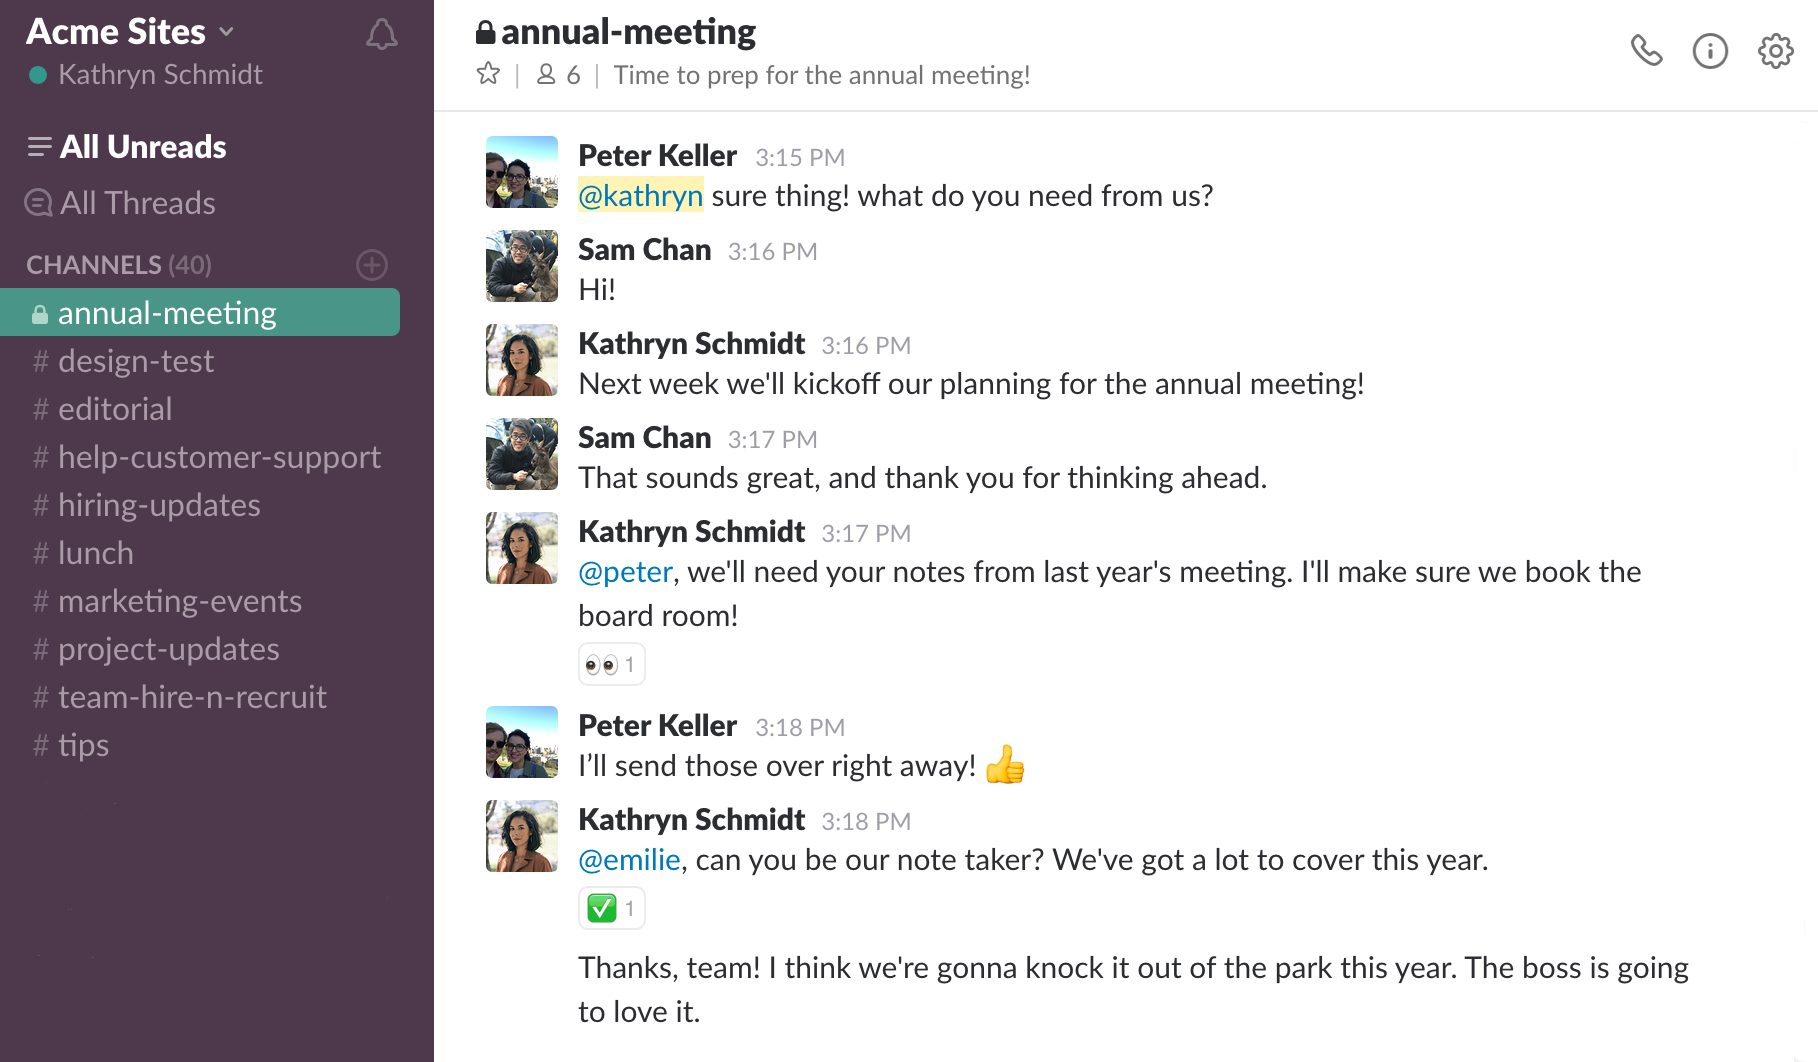
\includegraphics[scale=0.2]{slack}
    \caption{Pantalla principal de Slack - \textcopyright\ Slack}
    \label{slackimage}
\end{figure}

\subsection{Documentación}
Para gestionar la documentación y todo el contenido que el equipo produzca a lo largo del tiempo, es necesario contar con un espacio común de alojamiento de archivos. Para esto se puede optar por utilizar el servicio de almacenamiento en la nube \textbf{Google Drive} \cite{googledrive}.\\

Todos han de tener acceso a dicho directorio online, y ahí se han de ir dejando los documentos que el equipo genere, como pueden ser:
\begin{itemize}
    \item Presentaciones para exponer en reuniones.
    \item Actas de reuniones.
    \item Bocetos de diseño de aplicaciones o de identidad visual.
    \item Calendario semanal actualizado.
\end{itemize}

\subsection{Seminarios y divulgación}
Otro aspecto importante a la hora de realizar un proyecto de este tipo son los seminarios. Los seminarios permiten realizar una presentación y explicación de algún tema o concepto concreto de cualquier área del conocimiento, y generalmente pueden ser para un público más conocedor del tema, o hacerlo más divulgativo para que puedan comprender sus contenidos personas de todos los ámbitos.\\

En un equipo formado por diferentes estudiantes y profesores, es importante dar a conocer conceptos o técnicas habituales en algunas ramas del conocimiento, con el fin de que todos conozcan, no en un nivel avanzado, aspectos importantes para el proyecto, y que a algunos miembros no les resulte extraño o desconocido lo que hacen.\\

Por medio de los seminarios, podemos explicar algo a todo el equipo, y existen diversas técnicas de creatividad que los pueden hacer partícipes en los seminarios, para así motivarlos más y que logren afianzar mejor los nuevos conocimientos.

\subsubsection{Catálogo de seminarios}
Existen multitud de métodos de generación de ideas, que abarcan procesos de análisis, investigación/descubrimiento y definición de estrategias:

\begin{itemize}
    \item Card sorting
    \item Design Thinking
    \item Brainstorming
    \item SCAMPER
    \item Business Model Canvas
\end{itemize}

En esta documentación no vamos a hablar de cada uno de esos métodos, sino que nos centraremos en el que consideramos más interesante y que usaremos en este proyecto, el \textbf{Design Thinking}

\subsubsection{Design Thinking}
Una de las técnicas de creatividad más útiles es la del \textit{Design Thinking}. Tal y como podemos ver en \cite{designthinkinglink}, podemos definirlo como:\\

\textit{``Es un método para generar ideas innovadoras que centra su eficacia en entender y dar solución a las necesidades reales de los usuarios. Proviene de la forma en la que trabajan los diseñadores de producto. De ahí su nombre, que en español se traduce de forma literal como "Pensamiento de Diseño", aunque nosotros preferimos hacerlo como "La forma en la que piensan los diseñadores".''}\\

El Design Thinking es una herramienta muy visual que le da importancia a la experimentación y el prototipado. Su eficacia radica en la capacidad de entender y dar solución a las necesidades reales de los usuarios.\\

Es una técnica muy recomendable y que cada vez se usa más, por lo que es muy recomendable ponerla en práctica con el equipo, ya que puede ser un gran estímulo para obtener ideas, además de que ayuda a que el equipo se conozca mejor y haya más complicidad entre integrantes.

\section{Conclusión}
En este capítulo se han descrito las técnicas y actividades que se pueden realizar para gestionar un equipo multidisciplinar. Los resultados obtenidos tras su aplicación pueden verse en el capítulo \ref{ch:conclusiones}, así como un análisis de los mismos.
